\documentclass[a4paper,12pt,headsepline]{article}
\usepackage{paralist}		% List environment
\usepackage{color}		% For colored text
\usepackage{times}
\usepackage{amsfonts}		% Additional math fonts
\usepackage{amsmath}		% Math symbols
\usepackage{latexsym}
\usepackage{graphicx}		% For including images
% \usepackage{listings}		% If listings are needed
% \usepackage{wrapfig}		% To wrap images
% \usepackage{algorithmic}	% Nice algorithm environment
% \usepackage{algorithm}
%\usepackage{fullpage} % Use the full page
\usepackage{fancyhdr}
\usepackage{graphicx,calc} % for pix
\usepackage{subfigure}
\usepackage{color}    % for coloured text
\usepackage{ifthen}
\usepackage{paralist}
\usepackage{times}
\usepackage{longtable}
\usepackage{colortbl}
\usepackage{nomencl}
\usepackage{multicol} % multiple columns

\renewcommand{\vec}[1]{\mathbf{#1}}
\newcommand{\mat}[1]{\mathtt{#1}}
\newcommand{\pinv}{^{+}}
\newcommand{\inv}{^{-1}}
\newcommand{\trans}{^{\!\top}}
\newcommand{\invtrans}{^{-\!\top}}
\newcommand{\myref}[1]{(\ref{#1})}
\newcommand{\myeqref}[1]{Eq.~\myref{#1}}
\newcommand{\myfigref}[1]{Fig.~\ref{#1}}
\newcommand{\mychapterref}[1]{Chapter~\ref{#1}}
\newcommand{\mysecref}[1]{Section~\ref{#1}}
\newcommand{\myalgoref}[1]{Algorithm~\ref{#1}}

% Change the appearance of the header. Here \MakeUppercase is hard-coded,
% so renewing this command allows to elegantly change the header appearance.
\renewcommand{\MakeUppercase}{\scshape}

\author{Simon Schaefer}

% Header definition.
\pagestyle{fancy}
\fancyhf{}
\rhead{Simon Schaefer}
\lhead{Task-Aware-Downscaling for Image and Video Domain}
\rfoot{\thepage}

% The first pages shall be empty, even no page numbering
\begin{document}
\pagestyle{empty} % even no page number

% Title page, modify accordingly
\begin{titlepage}

\thispagestyle{empty}

\fancypagestyle{empty}{
\lhead{
\includegraphics[height=1.5cm]{figures/ethlogo_black}}
\renewcommand{\headrulewidth}{0.0pt}
\rhead{\vspace*{-0.2cm}
\includegraphics[height=1.4cm]{figures/cvl}}
\fancyfoot{}
}

\vspace*{2cm}
\begin{center}
\Huge{\textbf{Efficient Task Aware Super-Resolution and Colorization}\\}
\LARGE{\textbf{For Image and Video Domain}\\[1cm]}

\large{Semester Project\\[0.8cm]}
\LARGE{Simon Schaefer\\}
\end{center}

\vspace*{2cm}
\begin{center}
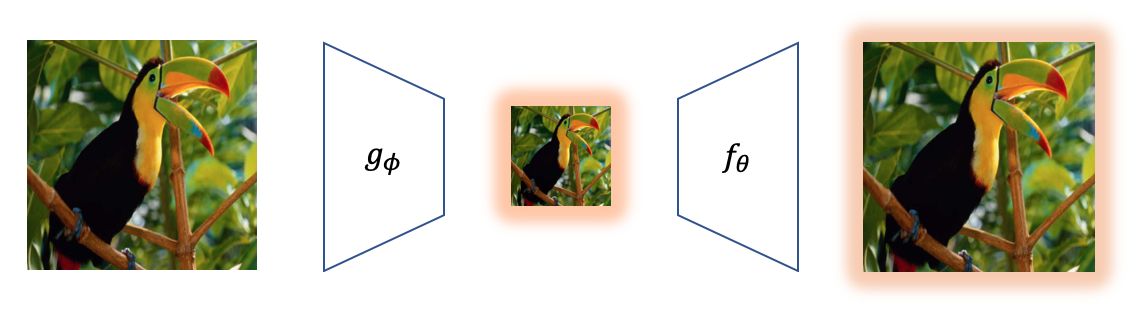
\includegraphics[height=4cm]{figures/titlepage}
\end{center}

\vfill
\begin{center}
\begin{tabular}{ll}
\Large{\textbf Advisor:} & \Large{Dr. Radu Timofte, Shuhang Gu}\\
\Large{\textbf Supervisor:} & \Large{Prof.~Dr.~Luc van Gool}\\
			    & \small{Computer Vision Laboratory}\\
			    & \small{Department of Information Technology and Electrical Engineering}\\
\end{tabular}
\end{center}

\begin{center}
\today\\
\end{center}


\end{titlepage}

% !Tex root = main.tex
\newpage
\section*{Abstract}
\addcontentsline{toc}{section}{Abstract}
\noindent The abstract gives a concise overview of the work you have done. The reader shall be able to decide whether the work which has been done is interesting for him by reading the abstract. Provide a brief account on the following questions:

\begin{itemize}
 \item What is the problem you worked on? (Introduction)
 \item How did you tackle the problem? (Materials and Methods)
 \item What were your results and findings? (Results)
 \item Why are your findings significant? (Conclusion)
\end{itemize}

\noindent The abstract should approximately cover half of a page, and does generally not contain citations.

\newpage

\chapter*{Acknowledgements}


\pagestyle{fancy}
\pagenumbering{Roman}

% Insert table of contents
\newpage
\tableofcontents
% Insert list of figures.
\newpage
\listoffigures
% Insert list of tables
%\newpage
%\listoftables

\pagenumbering{arabic}

%% ----------------------------------------------------------------------------
% Actual text
%% ----------------------------------------------------------------------------
\newpage
\section{Introduction}
\label{sec:Introduction}
With the rise of deep learning in image processing super-resolution (SR) and image
colorization (IC) in both the image and the video domain have received significant
attention \cite{DLFISRAS}. While SR aims to reconstruct a high-resolution (HR)
image from a low-resolution (LR) image, image colorization deals with the
transformation from an uncolored, grayscale (GR) image to a RGB colored
(COL) image.
However, in most of the recent works (e.g. \cite{AFPATSISR}, \cite{ESRGAN},
\cite{RBPNFVSR}, \cite{LFVSRTHROFE}) the problem of downscaling and upscaling
or decolorization and colorization are regarded as seperate problems although
upscaling often is preceded by downscaling, leading to a loss of information
from the downscaling process which makes the inverse problem of SR highly
ill-posed \cite{TAID}. Despite of the large progress in SR in the last years
(\cite{DLFISRAS}) very specific details therefore often cannot be reconstructed,
when interpolation is used for downsampling. However, as shown in
\myfigref{fig:shrb_vs_shrt_x4} the downsampling method has a large impact on
the performance of the subsequent upscaling task.

\begin{figure}[!htbp]
	\centering
	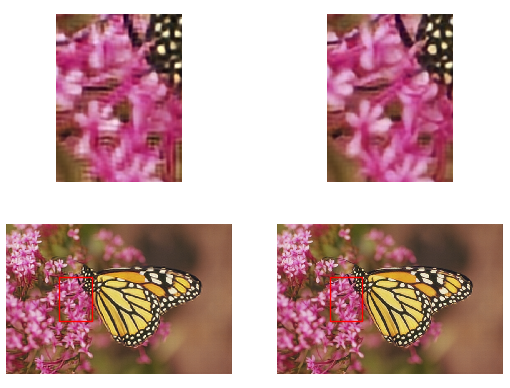
\includegraphics[width=6cm]{figures/shrb_vs_shrt_x4}
  
\includegraphics[width=6cm]{figures/cvl}
	\caption{Comparison between an upscaled image based on bicubic downsampled
  (left) and task-aware downsampled (right) LR image applied on the same model
  with upscaling factor 4, for the image-domain, SET 14 dataset, and video
  domain, CALENDAR dataset. }
  \label{fig:shrb_vs_shrt_x4}
\end{figure}

As can be seen above a task-aware approach can dramatically improve the
performance of existing super-resolution models. However, the research on task-
aware downscaling methods is a very new field and therefore there still are
a lot of unresolved issues such as the effect of noise or the feasibility of
applying it in other domains.

\newpage
\subsection{Focus of this Work}
For this reason this work focuses on Task-Aware-Downscaling (TAD) for several standard
computer vision problems such as super-resolution or colorization in both the
image and video domain, as recently purposed by Heewon Kim et. alt. (\cite{TAID})
for the image domain only. Therefore the goals of this work are the following

\begin{itemize}
  \item reimplement and evaluate the TAD framework purposed in (\cite{TAID})
  \item improve the TAD framework especially with regards on accuracy
  (PSNR) and speed in the image domain
  \item evaluate the effect of external effects such as noise on the TAD
  framework
  \item extend the TAD framework to the video domain
\end{itemize}

By that to the best of our knowledge this work is the first one using deep
learning for downscaling in the video domain.

\subsection{Thesis Organization}
After the problem statement \mychapterref{sec:Introduction} related works are
introduced for both the image and video domain \mychapterref{sec:RelatedWork}.
\mychapterref{sec:Approach} explains the methods that are used in order to
achieve the goals described above and which are evaluated in
\mychapterref{sec:ExperimentsandResults}. A final discussion of the results
as well as an outlook on further work can be found in
\mychapterref{sec:Discussion} and \mychapterref{sec:Conclusion}.
Further visualization and experiments are shown in the abstract.

% Give an introduction to the topic you have worked on:
%
% \begin{itemize}
%  \item \textit{What is the rationale for your work?} Give a sufficient description of the problem, e.g. with a general description of the problem setting, narrowing down to the particular problem you have been working on in your thesis. Allow the reader to understand the problem setting.
%  \item \textit{What is the scope of your work?} Given the above background, state briefly the focus of the work, what and how you did.
%  \item \textit{How is your thesis organized?} It helps the reader to pick the interesting points by providing a small text or graph which outlines the organization of the thesis. The structure given in this document shows how the general structuring shall look like. However, you may fuse sections or change their names according to the requirements of your thesis.
% \end{itemize}

\newpage
\section{Related Work}
\label{sec:RelatedWork}
In the following previous work in super-resolution, colorization and
task aware-downscaling are presented. At the end of each section the models
used for comparison and evaluation of the the underlying approach are further
explained in detail. Thereby the models were selected based on several criterias
performance compared to the state-of-the-art, the use as benchmark in related
papers and availability of (pretrained) models.

\subsection{Super-Resolution in Image Domain}
The problem of SR in the image domain is called \ac{SISR} and is shown in
\myfigref{fig:sisr_problem}. A lot of approaches have been
tried in order to cope with the \ac{SISR} problem. While early approaches such as
bicubic and Lanczos \cite{LFIOATD} tackle the problem using simple deterministic
filters which are computational cheap but produce blurry results and lack in
high frequency details, more recent approaches approach the problem using
example-based methods such as sparse encoding or deep learning methods.

\begin{figure}[!htbp]
	\centering
	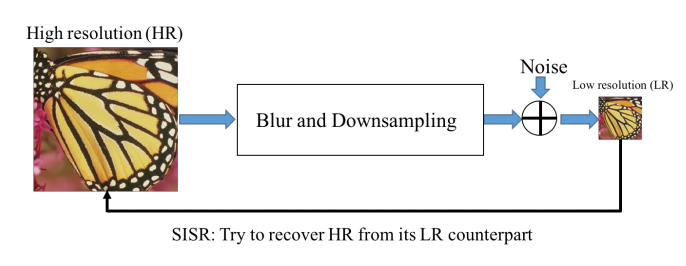
\includegraphics[width=10cm]{figures/sisr_problem}
	\caption{General SISR problem  according to \cite{DLFSISRABR}.}
  \label{fig:sisr_problem}
\end{figure}

Sparsity-based techniques assumes the \ac{LR} image to be transformable in another
domain (usually a dictionary of image atoms \cite{SARPFTTAISAIP}) and tries to
find correspondences between the \ac{LR} and \ac{HR} patches in the transformed space, as
implemented in \cite{IDASRBASDSAAR}. However, these techniques usually are
very computationally expensive. Among other learning based approaches such as
the use of random forests \cite{FAAIUWSRF}, in-place example regression models
\cite{FISRBOIPER} or adjusted anchored neighborhood regression \cite{AANRFFSR},
in terms of accuracy applying CNN based approaches have shown the largest success.
\footnote{An overview of various other deep learning based approaches for SISR
can be found in \cite{DLFSISRABR}.}
Dong et al. \cite{LADCNFISR} trained a shallow CNN end-to-end to build the HR
image based on a bicubicly upscaled LR image. This approach was improved by Kim
et al. \cite{AISRUVDCN} (VDSR) using a deeper network (20 layers) and cascading
small filters many times in a deep network structure to exploit contextual
information over large image regions in an efficient way. By advancing the
network model VDSR was further improved by Lim et al. \cite{EDRNFSISR} which
got the best results in the NTIRE2017 Super-Resolution Challenge \cite{NTIRE2017}.

\begin{figure}[!htbp]
	\centering
	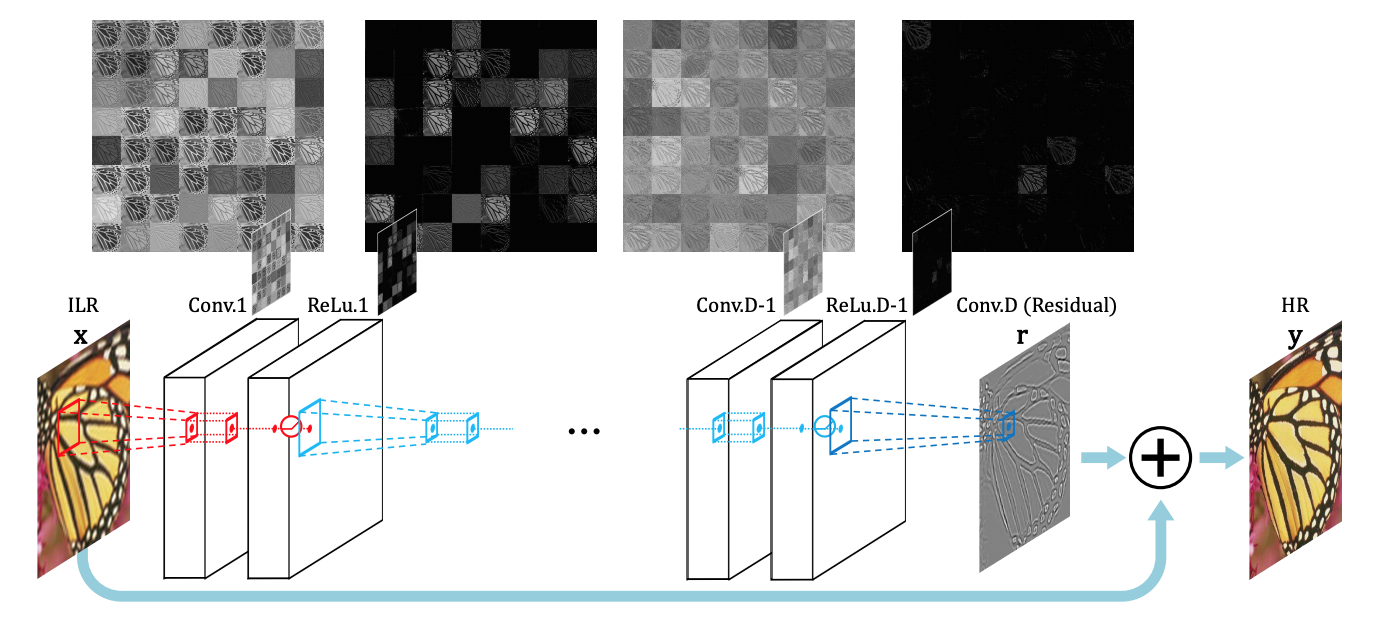
\includegraphics[width=10cm]{figures/vdsr}
	\caption{Overview of VDSR network design \cite{AISRUVDCN}.}
  \label{fig:vdsr}
\end{figure}

\subsection{Super-Resolution in Video Domain}
\ac{VSR} combines information from multiple adjacent LR frames
to take temporal information into account, leading to higher quality results.
Takeda et al. \cite{SRWESME} apply a 3D kernel regression on a patch of adjacent
\ac{LR} frames to implicitly encounter temporal information. Since purposed by
Caballero et al. \cite{RTVSRWSTNAMC} end-to-end approaches including motion
compensation such as the CNN framework from \cite{RTVSRWSTNAMC} have large success
in the VSR area. Liu et al. \cite{RVSRWLTD} added temporal addaptivity to the
framework to be able to aggregate the resulting \ac{HR} frame based on a weighted
sum of several estimates as well as a varying number of input LR frames. Sajjadi
et al. \cite{FRVSR} purposed a frame-recurrent architecture iteratively using
the previously inferred \ac{HR} frames for the subsequent prediction. Wang et al.
\cite{LFVSRTHROFE} (SOFVSR) implemented an end-to-end trainable approach to predict
both, the \ac{HR} frame as well as the HR optical flow. Therefore, first the HR
optical flow is inferred in a coarse-to-fine manner, then motion compensation is
performed according to the HR optical flows and finally, the compensated LR
inputs are fed to a super-resolution network to generate the HR frame estimate
(comp. \myfigref{fig:sofvsr}).

\begin{figure}[!htbp]
	\centering
	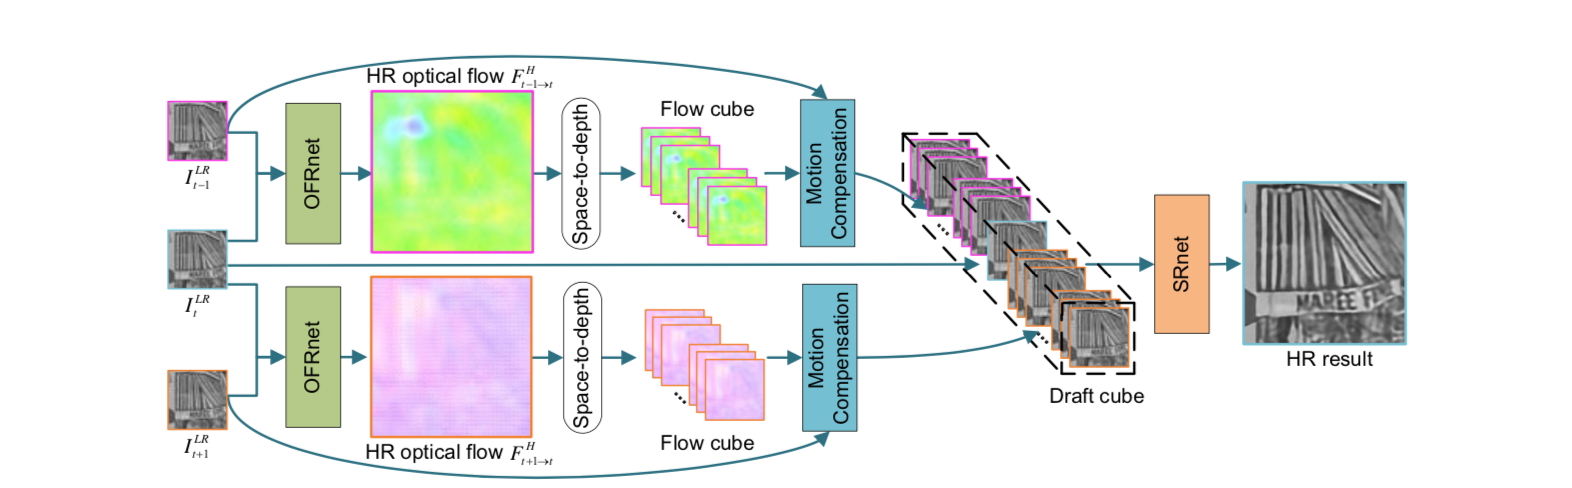
\includegraphics[width=10cm]{figures/sofvsr}
	\caption{Overview of SOFVSR pipeline \cite{LFVSRTHROFE}.}
  \label{fig:sofvsr}
\end{figure}

\subsection{Colorization}
Image colorization methods can be categorized in two categories: Non-parametric
approaches, such as \cite{ICUSI}, model the correspondence between the grayscale
and the colored image by finding analogeous regions in reference image(s),
while parameteric models learns this correspondence from large datasets,
transforming the colorization problem into a regression problem. Zhang et al.
\cite{CIC} (CIC) purpose posing colorization as a classification task and use
class-rebalancing at training time to increase the diversity of colors in the
result, using the CNN shown in \myfigref{fig:cic} and not requiring any
user-interaction.

\begin{figure}[!htbp]
	\centering
	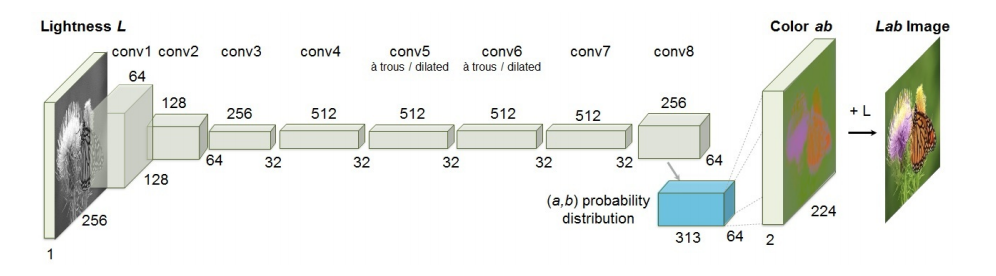
\includegraphics[width=10cm]{figures/cic}
	\caption{Overview of CIC network design \cite{CIC}.}
  \label{fig:cic}
\end{figure}

\subsection{Task-Aware-Downscaling}
Over all of the problems stated above most of the approaches merely take into
account one side of the process, e.g. by fixing the transformation HR to LR
to bicubic interpolation in order to large amount of training data and focusing
on estimating the inverse transformation. Kim et al. \cite{TAID} (TAID) purpose taking
into account the downscaling method in order to improve the upscaling performance,
by training an autoencoder in an end-to-end manner while the latent space
representation again is an image of same size as the LR image. The loss function
thereby contains both the difference between the decoded SHR and the original HR
image as well as the difference between the encoded SLR and the bicubic
interpolated LR image, such that the SLR image is a humanly understandable
representation. Next to SISR the approach is shown to be applicable for large
scale factor up to 128 as well as for colorization.


% Describe the other's work in the field, with the following purposes in mind:
%
% \begin{itemize}
%  \item \textit{Is the overview concise?} Give an overview of the most relevant work to the needed extent. Make sure the reader can understand your work without referring to other literature.
%  \item \textit{Does the compilation of work help to define the ``niche'' you are working in?} Another purpose of this section is to lay the groundwork for showing that you did significant work. The selection and presentation of the related work should enable you to name the implications, differences and similarities sufficiently in the ``discussion'' section.
% \end{itemize}

\newpage
\section{Approach}
\label{sec:Approach}



\begin{figure}[!htbp]
	\centering
	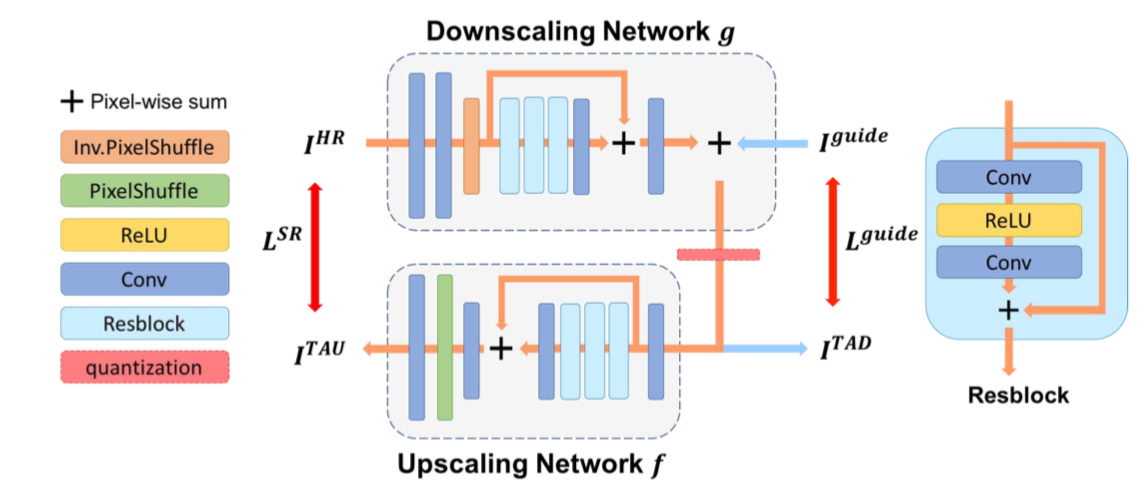
\includegraphics[width=10cm]{figures/tad_overview}
	\caption{Overview of TAID autoencoder network design \cite{TAID}.}
  \label{fig:tad_overview}
\end{figure}


% The objectives of the ``Materials and Methods'' section are the following:
% \begin{itemize}
%  \item \textit{What are tools and methods you used?} Introduce the environment, in which your work has taken place - this can be a software package, a device or a system description. Make sure sufficiently detailed descriptions of the algorithms and concepts (e.g. math) you used shall be placed here.
%  \item \textit{What is your work?} Describe (perhaps in a separate section) the key component of your work, e.g. an algorithm or software framework you have developed.
% \end{itemize}

\newpage
\section{Experiments and Results}
\label{sec:ExperimentsandResults}
In order to test the previously described \ac{TAD} approach several experiments
were performed, to find the optimal model for both the \ac{SISR} and \ac{IC}
tasks, to show the impact of the L1 ball on the model's robustness against
perturbations as well as evincing the feasibility of applying the \ac{TAD}
method in the video domain.

\begin{figure}[!htbp]
	\centering
	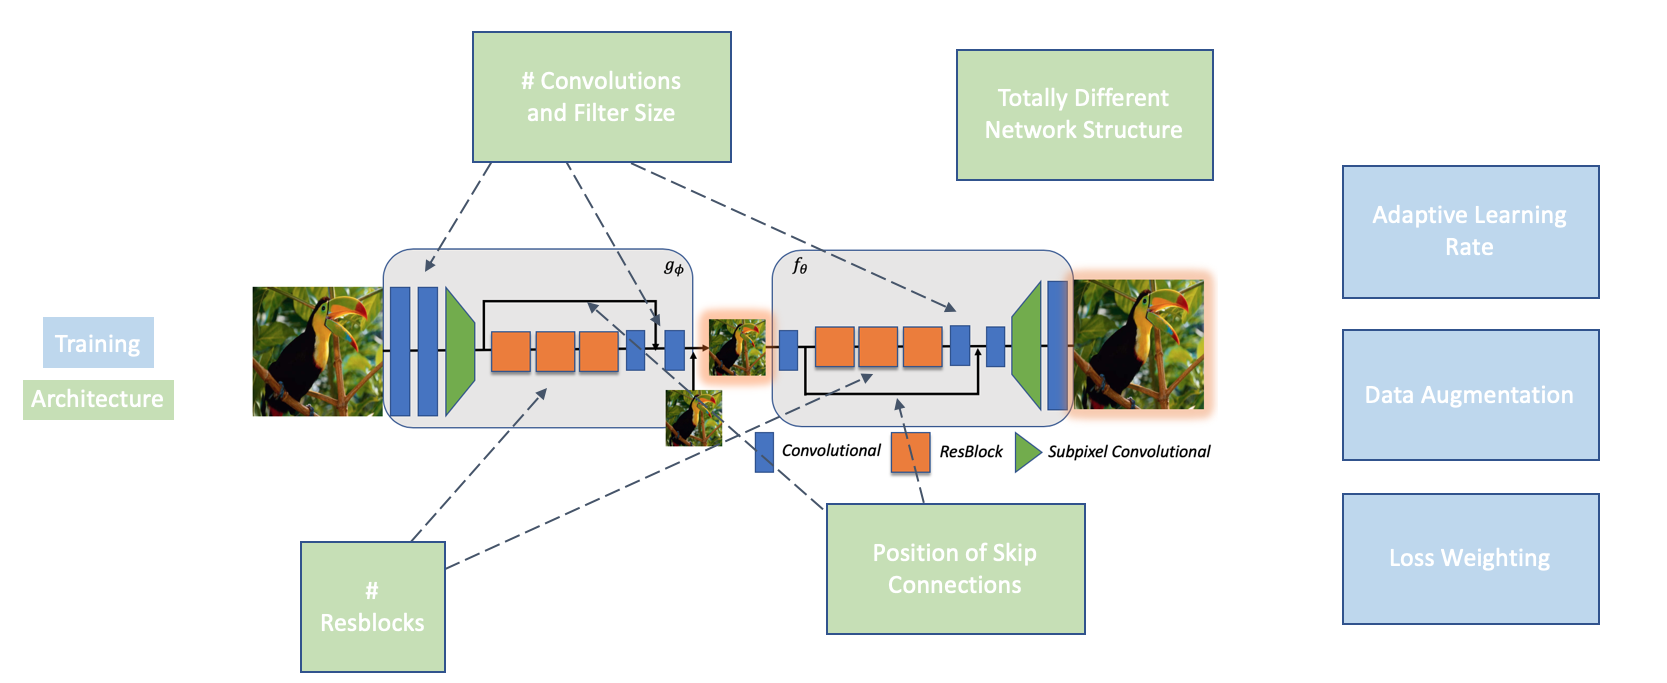
\includegraphics[width=14cm]{figures/model_adaptions}
	\caption{Model and Training adaptions during experiments in comparison
  to the baseline model by \cite{TAID}.}
  \label{fig:model_adaptions}
\end{figure}

As shown in \myfigref{fig:model_adaptions} a bunch of adjustments to the
baseline model (by \cite{TAID}) were tried for analysing the coherence between
the model complexity and its reconstruction performance. Thereby very small
architectures (6 layers) as well as comparable large architectures
(19 layers) were tested (baseline model has 10 layers), spanning
from $375.926$ to $1.299.126$ parameters. Since the model already is quite
shallow the removal of each layer had an impact on the resulting performance,
therefore especially the number of \textit{Resblocks} (two convolutional layers
and ReLU) has a huge impact on the reconstruction accuracy. Next to adaptions
to the baseline architecture completly new architectures have been tested, such
as networks without any residual pass (so no Resblocks) but convolutional layers
with either constant or varying (first increasing then decreasing) number of
filters (up to 256) have been used.
\newline
Next to several architectures the baseline model was improved by advancing the
training procedure. Next to enhancing the loss function as discussed in
\mysecref{sec:Approach_LF} instead of a constant an linearly annealing learning
rate was used, starting at $4*10^{-4}$ and annealing by factor $\gamma = 0.25$
after $20$, $100$ and again after $200$ training epochs. Adam optimizer was used
with $\beta = (0.9, 0.999)$, $\epsilon = 10^{-8}$, gradient clipping and  zero
weight decay.
\newline
To guarantee comparability to other super-resolution and colorization paper
in the image domain the model was trained using the DIV2K training dataset
(\cite{DIV2K}), while validated on the SET5 (\cite{SET5}), SET14 (\cite{SET14}),
BSDS100 (\cite{BSDS100}), URBAN100 (\cite{URBAN100}) and VDIV2K (\cite{DIV2K})
dataset. For similar reason for the video domain the model was pretrained using
DIV2K, actually trained on video clips from CDVL Database (Ntiaspen) and
validated on the widely known Vid4 dataset (Calendar, Foliage, Walk, City).
For improving generalization capabilities of the model and avoid overfitting
the image training data were also augmented (rotated, mirrored).
\newline
A complete list of the most important testing configurations and their results
can be found in the appendix.

\subsection{Impact of L1 Ball}
\label{sec:Experiments_EPS_BALL}



\subsection{Single-Image Super-Resolution}
\label{sec:Experiments_SISR}

\begin{enumerate}
\item different scales
\item very large scales
\item performance on other non-trained scales
\end{enumerate}

\subsection{Image Colorization}
\label{sec:Experiments_IC}

\subsection{Video Super-Resolution}
\label{sec:Experiments_VSR}

\begin{enumerate}
\item super-large scale for videos
\end{enumerate}

\subsection{Qualitative Improvements}
\label{sec:Experiments_QI}

\begin{enumerate}
\item gummibear image (TAD learns to downscale an image task-aware and thereby
can store information that are lost by simple downscaling (e.g. bilinear
interpolation, averaging colors). Therefore, possibly even image can restored
that are impossible to restore  using classic approaches, like exactly
similar gummibears.)
\end{enumerate}

% Describe the evaluation you did in a way, such that an independent researcher can repeat it. Cover the following questions:
% \begin{itemize}
%  \item \textit{What is the experimental setup and methodology?} Describe the setting of the experiments and give all the parameters in detail which you have used. Give a detailed account of how the experiment was conducted.
%  \item \textit{What are your results?} In this section, a \emph{clear description} of the results is given. If you produced lots of data, include only representative data here and put all results into the appendix.
% \end{itemize}

\newpage
\chapter{Discussion}
The discussion section gives an interpretation of what you have done \cite{day2006wap}:

\begin{itemize}
 \item \textit{What do your results mean?} Here you discuss, but you do not recapitulate results. Describe principles, relationships and generalizations shown. Also, mention inconsistencies or exceptions you found.
 \item \textit{How do your results relate to other's work?} Show how your work agrees or disagrees with other's work. Here you can rely on the information you presented in the ``related work'' section.
 \item \textit{What are implications and applications of your work?} State how your methods may be applied and what implications might be.
\end{itemize}

\noindent Make sure that introduction/related work and the discussion section act as a pair, i.e. ``be sure the discussion section answers what the introduction section asked'' \cite{day2006wap}.

\chapter{Conclusion}

List the conclusions of your work and give evidence for these. Often, the discussion and the conclusion sections are fused.


%% ----------------------------------------------------------------------------
% Bibliography
%% ----------------------------------------------------------------------------
\newpage
\bibliographystyle{plain}
\bibliography{references}

%% ----------------------------------------------------------------------------
% If Appendix is needed
%% ----------------------------------------------------------------------------
\newpage
\appendix
\section{Appendix}
\label{sec:Appendix}

In the appendix, list the following material:

\begin{itemize}
 \item Data (evaluation tables, graphs etc.)
 \item Program code
 \item Further material
\end{itemize}


\end{document}
